\documentclass[11pt,a4paper]{article}
\usepackage[margin=2.2cm]{geometry}
\usepackage{amsmath,amssymb}
\usepackage{siunitx}
\usepackage{booktabs}
\usepackage{xcolor}
\usepackage{microtype}
\usepackage{enumitem}
\usepackage{tcolorbox}
\usepackage{graphicx}
\definecolor{ink}{HTML}{14231B}\definecolor{accent}{HTML}{0F3D2A}
\tcbuselibrary{skins}
\newtcolorbox{key}{colback=accent!6,colframe=accent,boxrule=0.6pt,arc=2pt,left=6pt,right=6pt,top=4pt,bottom=4pt}
\sisetup{per-mode=symbol,group-separator={\,}}
\setlength{\parindent}{0pt}\setlength{\parskip}{6pt}
\renewcommand{\arraystretch}{1.25}

\title{\textbf{Slide 5: gain stage}\\\large Gain of 4.9, referenced to the mid-rail}
\author{ADS7057 test board v3 \quad ---\quad study notes}\date{}
\begin{document}\maketitle\vspace{-1.2em}
\section{The circuit}
U1B is a non-inverting amplifier. R3 feeds part of the output back to the $-$ input and R4 returns the other end to VMID5 ($\SI{1.65}{V}$), not to ground.
\begin{center}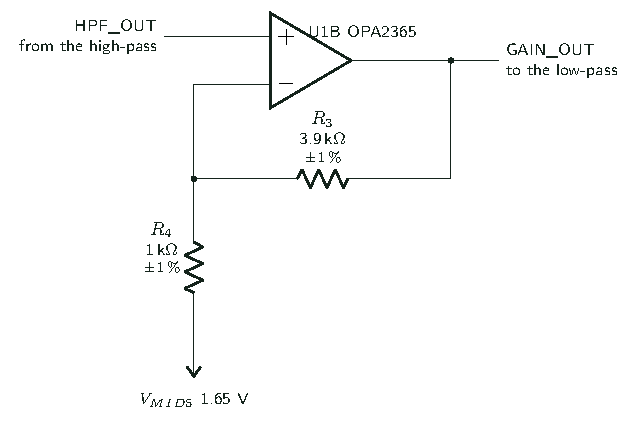
\includegraphics[width=0.7\textwidth]{s05_circuit.pdf}\end{center}

\section{Gain from the op-amp equation}
Let $v$ be the deviation from VMID5. The feedback divider gives the $-$ input
\[
v_-=\beta\,v_o,\qquad \beta=\frac{R_4}{R_3+R_4}=\frac{1\,\text{k}\Omega}{4.9\,\text{k}\Omega}=0.204 .
\]
The op-amp equation with finite gain $A$ is $v_o=A\,(v_{in}-v_-)=A\,(v_{in}-\beta v_o)$. Solve for $v_o$:
\[
\frac{v_o}{v_{in}}=\frac{A}{1+A\beta}=\frac{1}{\beta}\cdot\frac{1}{1+\dfrac{1}{A\beta}}
\;\xrightarrow{A\to\infty}\;
\boxed{G=\frac1\beta=1+\frac{R_3}{R_4}=1+\frac{3.9}{1}=4.9}\quad(\SI{13.8}{dB}).
\]
\textbf{The DC point.} Because R4 returns to VMID5, the deviation equation holds for the total voltages too:
\[
V_o-V_{MID5}=G\,(V_{in}-V_{MID5}).
\]
A signal that rests at VMID5 (the high-pass output does) leaves the output at VMID5 as well. The gain applies only to the burst, and DC passes at $\times1$. If R4 went to ground, the stage would amplify the \SI{1.65}{V} rest level to \SI{8.1}{V} and clip.

\section{Bandwidth}
With $A=\omega_t/s$ ($\mathrm{GBW}=\SI{50}{MHz}$), the finite-gain factor is $1/(1+s/(\beta\,\omega_t))$. The closed-loop pole is at
\[
\beta\cdot\mathrm{GBW}=0.204\times\SI{50}{MHz}=\SI{10.2}{MHz}.
\]
At \SI{250}{kHz} the loss is $-0.0003$\,dB. The stage is accurate across the band.

\section{Headroom: what clips first}
The output can swing about \SI{0.1}{V} from each rail. That gives $\pm(1.65-0.1)=\SI{1.55}{V}$ around VMID5. The largest input amplitude before clipping is
\[
\frac{1.55}{4.9}=\SI{0.32}{V}\ \text{at the gain-stage input.}
\]
The simulation, which includes the bias-T, the high-pass and the gain, clips at about \SI{0.35}{V} at the head output (total gain 4.45 from the head to GAIN\_OUT at 250\,kHz). A typical recorded event is \SI{120}{mV}, so the margin is $2.9\times$. The largest of the seven events was \SI{236}{mV} peak to peak, about \SI{118}{mV} peak, on the perfboard. The new head loses less, so it reads about 25\,\% higher (\SI{150}{mV}). The margin for that event is about $2.3\times$.

\begin{center}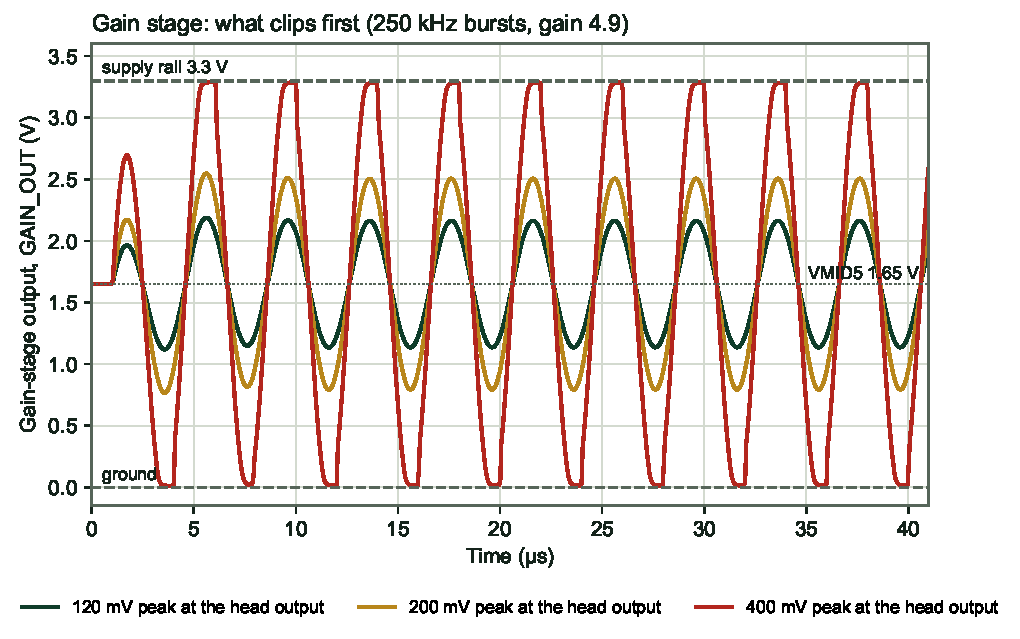
\includegraphics[width=0.78\textwidth]{s05_graph.pdf}\end{center}
The \SI{120}{mV} burst reaches \SI{2.2}{V} and stays inside the rails. The \SI{200}{mV} burst reaches \SI{2.55}{V}. The \SI{400}{mV} burst flat-tops at both rails.

\section{Tolerance and noise}
\begin{itemize}[nosep]
\item $R_3,R_4$ are $\pm1\,\%$ (C23018, C21190). Worst case $G=4.82$ to $4.98$ ($\pm1.6\,\%$, about $\pm0.14$\,dB).
\item Noise of this stage, referred to its input: the op-amp \SI{4.5}{nV/\sqrt{Hz}} and $R_3\parallel R_4=\SI{0.8}{k\ohm}$ (\SI{3.6}{nV/\sqrt{Hz}}) add to about \SI{5.8}{nV/\sqrt{Hz}}. Over \SI{400}{kHz} that is $\approx\SI{3.7}{\micro V}$. The head's noise (\SI{100}{\micro V} at its output) dominates.
\item Why 4.9: a \SI{120}{mV} event fills about 5 times more ADC codes than with unity gain, and the stage still clips only above $\SI{0.35}{V}$. A change is one resistor (R3).
\end{itemize}
\end{document}
